\scanpage{100}
% archive foliation: 102
\uline{Cor} Supposons $k$ principal \inserted{$2$-régulier}, $k_0=k/2k$ un corps.
Alors les $(M,\sigma)$ \inserted{\unsure{cat. des}} précédents
\unsure{équiv. à} celles des paires $(P,Q,\deleted{\unsure{\bar p,\bar q,m}})$ où $P,Q$ libres de rg $1$,
et $\deleted{\unsure{p}}m\subset\underbrace{P/2P}_{p}\oplus\underbrace{Q/2Q}_{q}$ un espace vectoriel sur $k_0$,
\deleted{\unsure{de M, qui}}
qui est soit nul, soit une droite $\ne p,q$ (\unsure{droites coordonnées}).

\uline{Cor} Cela donne une description des classes de conjugaison,
d'éléments de $\mathrm{Gl}(2,k)^{\deleted{\unsure{*}}}$ qui sont d'ordre $2$ exactement, et
distincts de $\{\pm1\}$ : il y \deleted{\unsure{en a}} \inserted{celle de}
$\begin{pmatrix}1&0\\0&-1\end{pmatrix}$ (correspondant au
cas $m=0$), puis \uline{une} \deleted{famille, \unsure{indexée} par les \unsure{points de}
$\unsure{\mathbb P|\mathbf P}^1(k_0)$ distincts de $0,\infty$ (en supposant que
$k^\times\to k_0^\times$ est surjectif \unsure{sinon la classification sera plus fine})}
\margin{$\unsure{k'^\times\to k_0'^\times}$ \unsure{surj.}}
\unsure{en fait bien de} $P/2P\unsure{\to}Q/2Q$ en revenant au choix d'une base de $P,Q$.

\unsure{Plus} concrètement :
\[
P=k,\ Q=k,\ m=\text{diagonale de }k_0\oplus k_0\quad\text{i.e.}
\]
\[
M'=(2k\oplus2k)+\text{diag. de }k\oplus k
=\{(x,y)\mid x-y\in2k\}
\]
donc on peut prendre base de $M'$
\[
\unsure{e_0|u}=(2,0),\quad\unsure{e_1|v}=(1,1),\quad
\text{d'où}\quad-\unsure{e_0|u}+2\unsure{e_1|v}=(0,2)=\operatorname{sym}(\unsure{e_0|u})
\]
\margin{\figure{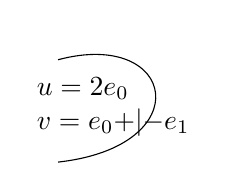
\begin{tikzpicture}\node[align=left] at (0,0) {$u=2e_0$\\$v=e_0\unsure{+|-}e_1$};\draw(-.7,.6)..controls(.8,1)and(1.1,-.5)..(-.7,-.7);\end{tikzpicture}}}
On trouve
\[
\sigma\unsure{e_0|u}=\unsure{e_0|u},\quad
\sigma\unsure{e_1|v}=(1,-1)=e_1-\operatorname{sym}\unsure{e_1|v}=\unsure{e_0-e_1|u-v}
\]
i.e. la matrice de $\sigma$ p.r. à $(\unsure{u,e_1|u,v})$ est
\[\begin{pmatrix}1&1\\0&-1\end{pmatrix}\]

Dans le cas $k=\mathbb Z$, c'est la matrice de la réflexion p.r. la
diagonale $0,e_0$ de l'hexagone régulier,
les \unsure{pts.|fl.} de l'hexagone étant rapportés à un
syst. de coordonnées obliques ayant comme base
deux sommets consécutifs $u$ $v$ ($M$ est le réseau
engendré par \unsure{l'ens|l'un} des sommets).
\figure{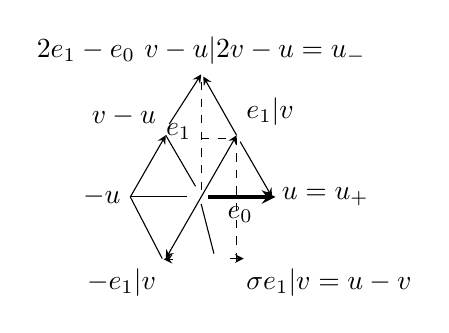
\begin{tikzpicture}[scale=.9,>=stealth]
\draw[->](-1,0)--(-.5,.87);\draw(-.5,.87)--(-.08,.15);
\draw[->](-.45,1.03)--(0,1.73);\draw[->](.5,.87)--(.03,1.7);
\draw[->](.55,.78)--(1,0);\draw[->](.4,-.87)--(.6,-.87);
\draw[->](-.4,-.88)--(-.53,-.88);\draw(-.55,-.87)--(-1,0);
\draw[->](0,0)--(.5,.87);\draw[->](0,0)--(-.5,-.87);
\draw[->,very thick](.1,0)--(1.05,0);\draw(-1,0)--(-.2,0);
\draw[dashed](0,.1)--(0,1.65);\draw[dashed](0,.82)--(.5,.82)--(.5,-.9);
\draw(0,-.1)--(.18,-.8);
\node[left]at(-1,0){$-u$};\node[above left]at(-.5,.87){$v-u$};
\node[above right]at(.5,.87){$\unsure{e_1|v}$};\node[right]at(1,0){$u=u_+$};
\node[below left]at(-.5,-.87){$-\unsure{e_1|v}$};
\node[below right]at(.5,-.87){$\sigma\unsure{e_1|v}=u-v$};
\node[left]at(0,.92){$\unsure{e_1}$};\node[below]at(.55,0){$e_0$};
\node[above]at(0,1.73){$\deleted{\unsure{2e_1-e_0}}\ \unsure{v-u|2v-u}=u_-$};
\end{tikzpicture}}

\uline{NB} Soit $u_+$ une base de $\pi_+$, $u_-$ une base de $\pi_-$, alors
\deleted{dans} On peut représenter $\sigma_{\mathbb R}$ pour la base $(u_+,u_-)$ de $\pi\otimes_{\mathbb Z}\mathbb R$,
par la matrice $\begin{pmatrix}1&0\\0&-1\end{pmatrix}$ le réseau $\pi$ étant identifié
à $\mathbb Z u_-+\mathbb Z u_+$ \deleted{$\unsure{\simeq\mathbb Z^2}$} dans le premier cas et dans le $2$\textsuperscript{d}
à l'ens des $xu_++yu_-$ tels que $x-y\in\mathbb Z$, $x,y\in\frac12\mathbb Z$.
\margin{$\sigma^2(e_1)=\sigma e_0-\sigma e_1=e_0-(e_0-e_1)=e_1$}
